%================================================================
\chapter{Theoretical Background}
%================================================================

%================================================================
\section{Theory}\label{sec:Theory}
%================================================================

%----------------------------------------------------------------
\subsection{Project Theory 1}\label{sec:project theory}
%----------------------------------------------------------------
This is \autoref{sec:project theory}.

Citation is done with \hologo{BibTeX} \cite[p.~100]{Sakurai}.

Cross-reference equations such as
\begin{equation}\label{eq:einstein}
    E = m c^2
\end{equation}
with \cref{eq:einstein}.

\autoref{fig:noise} brings the noise from the \textbf{figures folder}. 
\begin{figure}[H]
\begin{center}
\includegraphics[scale=0.5]{example} 
\end{center}
\caption{Make some noise.}
\label{fig:noise}
\end{figure}

\autoref{fig:happy} shows a happy animal found in the \textbf{Images folder}. 
\begin{figure}[H]
\begin{center}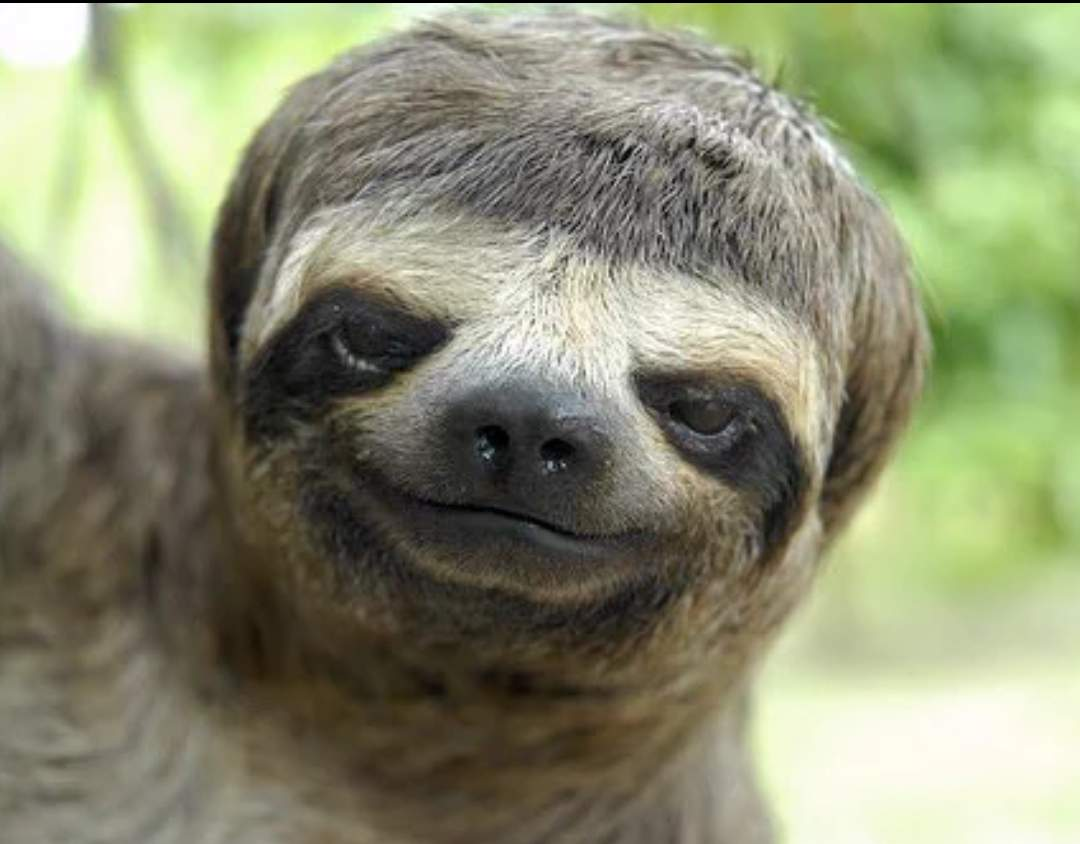
\includegraphics[scale=0.5]{latex-report/3_Images/Funny-Animal-Face} 
\end{center}
\caption{Sloths are arboreal mammals noted for slowness of movement and for spending most of their lives hanging upside down in the trees.}
\label{fig:happy}
\source{Insert image source here}
\end{figure}


\begin{figure}[H]
\centering
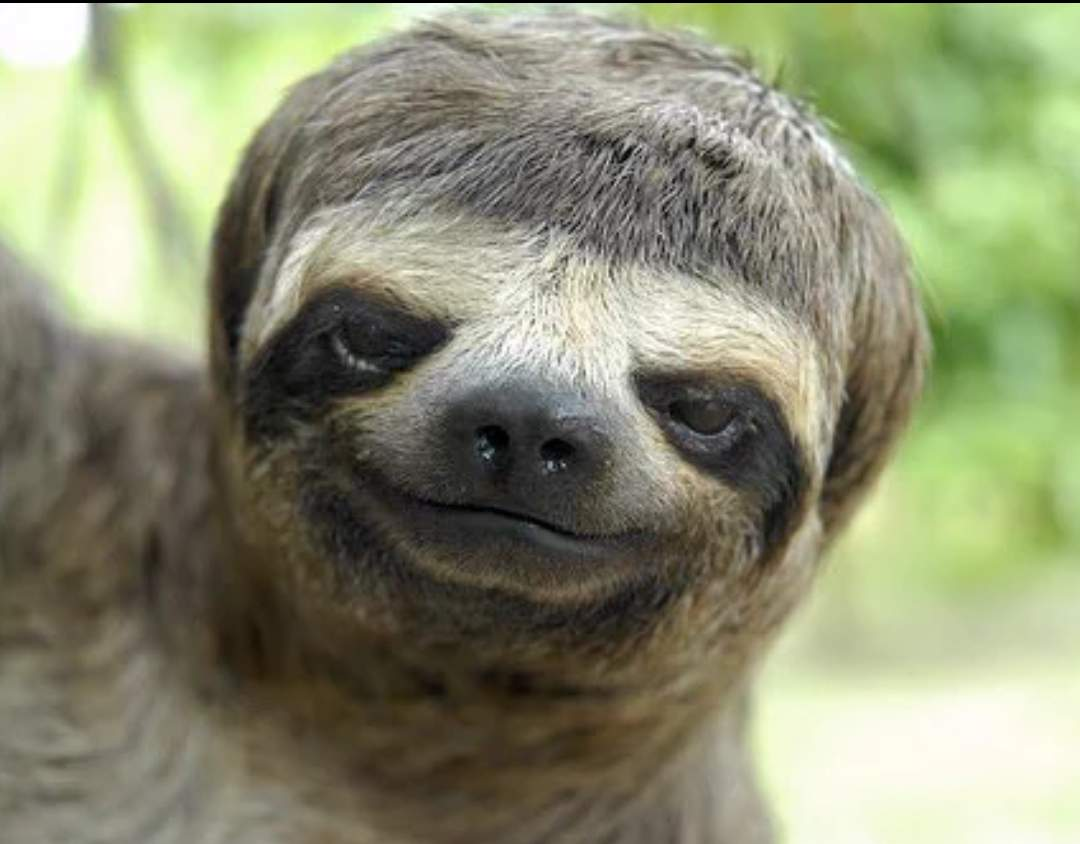
\includegraphics[width=0.5\textwidth]{latex-report/3_Images/Funny-Animal-Face} 
\caption{Sloths are arboreal mammals noted for slowness of movement and for spending most of their lives hanging upside down in the trees.}
\label{fig:happy2}
\source{Insert image source here}
\end{figure}



\autoref{tab:tab1} is from the \textbf{tables folder}. 
\begin{table}[H]
\caption{From pandas to latex.}
\centering
\rowcolors{2}{gray!25}{white}
\begin{tabular}{ccc}
\hline \hline
  $x$ &  $x^2$ &  $x^3$ \\
\hline \hline
0.250 &  0.062 &  0.016 \\
0.500 &  0.250 &  0.125 \\
0.750 &  0.562 &  0.422 \\
\hline \hline
\end{tabular}

\label{tab:tab1}
\end{table}

\autoref{tab:alternate} tabulates some values with alternating row colors.
\begin{table}[H]
\caption{Alternating background color for rows.}
\centering
\rowcolors{2}{gray!25}{white}
\begin{tabular}{ccc}
\hline
\hline 
$\alpha$ & $\beta$ & $\gamma$
\\
\hline 
\hline 
0.1 & 0.2 & 0.3
\\
0.4 & 0.5 & 0.6
\\
0.7 & 0.8 & 0.9
\\
\hline
\hline 
\end{tabular}
\label{tab:alternate}
\end{table} 

Table with nice rulers 

\begin{table}[h]
  \caption{Generic table with different sized rulers.}
  \footnotesize%
  \begin{center}
    \begin{tabular}{cccc}
      \toprule
      header1 & header2 & header3 & header4 \\
      \midrule
      col1 &  col2 & col3 & col4 \\
      col1 &  col2 & col3 & col4 \\
      col1 &  col2 & col3 & col4 \\
      col1 &  col2 & col3 & col4 \\
      \bottomrule
    \end{tabular}
  \end{center}
  \label{tab:tablerule}
\end{table}

Table with nice rulers and alternating rows

\begin{table}[h]
  \caption{Generic table with alternating rows and different sized rulers.}
  \footnotesize%
  \begin{center}
    \rowcolors{2}{white}{gray!15}
    \begin{tabular}{cccc}
      \toprule
      header1 & header2 & header3 & header4 \\
      \midrule
      col1 &  col2 & col3 & col4 \\
      col1 &  col2 & col3 & col4 \\
      col1 &  col2 & col3 & col4 \\
      col1 &  col2 & col3 & col4 \\
      \bottomrule
    \end{tabular}
  \end{center}
  \label{tab:tablerule2}
\end{table}

Table with nice rulers and alternating rows 2

\begin{table}[h]
  \caption{Generic table with alternating rows and different sized rulers.}
  \footnotesize%
  \begin{center}
    \rowcolors{2}{gray!15}{white}
    \begin{tabular}{cccc}
      \toprule
      header1 & header2 & header3 & header4 \\
      \midrule
      col1 &  col2 & col3 & col4 \\
      col1 &  col2 & col3 & col4 \\
      col1 &  col2 & col3 & col4 \\
      col1 &  col2 & col3 & col4 \\
      \bottomrule
    \end{tabular}
  \end{center}
  \label{tab:tablerule3}
\end{table}

Given
\begin{align*}
    f\colon \R \to \R,
    \intertext{magic happens}
    \int_{0}^{\infty} \mathrm{e}^{-x}\,\mathrm{d}x
\end{align*}


This is
\todo[inline]{Rewrite this!}

\section{Figures and Tables}

% Todonotes:
\begin{figure}[hbp]
    \centering
    \missingfigure{Three balls.}
    \caption[Three balls]{Three balls.}
\end{figure}


% Booktabs:
\begin{table}[htbp]
    \centering
    \begin{tabular}{@{}ll@{}}
        \toprule
        \textbf{Correct}               & \textbf{Incorrect}      \\
        \midrule
        \( \varphi \colon X \to Y \)   & \( \varphi : X \to Y \) \\[0.5ex]
        \( \varphi(x) \coloneqq x^2 \) & \( \varphi(x) := x^2 \) \\
        \bottomrule
    \end{tabular}
    \caption[Colons]{Proper colon usage.}
\end{table}

\begin{table}[htbp]
    \centering
    \begin{tabular}{@{}ll@{}}
        \toprule
        \textbf{Correct}     & \textbf{Incorrect}         \\
        \midrule
        \( A \implies B \)   & \( A \Rightarrow B \)      \\
        \( A \impliedby B \) & \( A \Leftarrow B \)       \\
        \( A \iff B \)       & \( A \Leftrightarrow B \)  \\
        \bottomrule
    \end{tabular}
    \caption[Arrows]{Proper arrow usage.}
\end{table}

% Tablefootnote and multirow:
\begin{table}[htbp]
    \centering
    \begin{tabular}{@{}ll@{}}
        \toprule
        \textbf{Correct}
        & 
        \textbf{Incorrect}
        \\
        \midrule
        \( -1 \) 
        & 
        -1
        \\[0.3ex]
        1--10
        &
        1-10
        \\[0.3ex]
        Birch--Swinnerton-Dyer conjecture
        &
        Birch-Swinnerton-Dyer conjecture
        \\[0.3ex]
        The ball \dash which is blue \dash is round.
        &
        \multirow{ 2}{*}{The ball - which is blue - is round.}
        \\[0.3ex]
        The ball---which is blue---is round. 
        &
        \\
        \bottomrule
    \end{tabular}
    \caption[Dashes]{Proper dash usage.}
\end{table}

It is now easy to tell that Birch and Swinnerton-Dyer are two people.

\begin{table}[hbtp]
    \centering
    \begin{tabular}{@{}*{2}{p{0.5\textwidth}}@{}}
        \toprule
        \textbf{Correct} &  \textbf{Incorrect}
        \\
        \midrule
        \enquote{This is an \enquote{inner quote} inside an outer quote}
        &
        "This is an 'inner quote' inside an outer quote"
        \\
        \bottomrule
    \end{tabular}
    \caption[Quotation marks]
    {Proper quotation mark usage.
    The \texttt{\textbackslash enquote} command chooses the correct
    quotation marks for the specified language.}
\end{table}